
\documentclass[11pt,letterpaper]{article}
\usepackage[letterpaper,top=0.78in,bottom=0.82in,left=0.84in,right=0.84in]{geometry}
\usepackage{mathtools}
\usepackage{libertinus-otf}
\usepackage{microtype}
\setmonofont{DejaVu Sans Mono}[Scale=MatchLowercase]
\usepackage{booktabs,longtable,tabularx,array,multirow}
\usepackage{graphicx,float,caption,subcaption}
\usepackage[dvipsnames,table]{xcolor}
\usepackage[most]{tcolorbox}
\usepackage{enumitem}
\usepackage{fancyhdr}
\usepackage{titlesec}
\usepackage{fvextra}
\usepackage{csquotes}
\usepackage[round,authoryear]{natbib}
\usepackage{doi}
\usepackage{hyperref}
\usepackage[nameinlink,capitalise,noabbrev]{cleveref}
\usepackage{xurl}
\usepackage{lastpage}
\usepackage{setspace}
\usepackage{etoolbox}
\usepackage{siunitx}
\usepackage{tikz}
\usetikzlibrary{arrows.meta,positioning,calc,fit,backgrounds}

% Fixed PDF trailer identifier for byte-reproducible release builds.
\AtBeginDocument{\special{pdf:trailerid [<ca1bec502620e6fde0c5cb753e33fffb><ca1bec502620e6fde0c5cb753e33fffb>]}}

\definecolor{FWNavy}{HTML}{13213A}
\definecolor{FWBlue}{HTML}{2E6173}
\definecolor{FWGold}{HTML}{A88345}
\definecolor{FWIvory}{HTML}{F7F3EA}
\definecolor{FWInk}{HTML}{1C2637}
\definecolor{FWMuted}{HTML}{5E6776}
\definecolor{FWLine}{HTML}{D8D0C3}
\definecolor{FWRed}{HTML}{8E3B46}
\definecolor{FWGreen}{HTML}{2E6B57}

\hypersetup{
  colorlinks=true,
  linkcolor=FWBlue,
  citecolor=FWBlue,
  urlcolor=FWBlue,
  pdftitle={Forecasting a World That Accelerates},
  pdfauthor={Vincent Boucher},
  pdfsubject={Acceleration-aware, constraint-limited, regime-switching forecasting},
  pdfkeywords={forecasting, AI, acceleration, regime switching, hindcasting, reliability, decision science}
}

\pagestyle{fancy}
\fancyhf{}
\fancyhead[L]{\sffamily\footnotesize\textcolor{FWMuted}{FORECASTING A WORLD THAT ACCELERATES}}
\fancyhead[R]{\sffamily\footnotesize\textcolor{FWMuted}{V2.0.0 · CEILING EDITION · JULY 28, 2026}}
\fancyfoot[L]{\sffamily\scriptsize\textcolor{FWMuted}{MONTREAL.AI · QUEBEC.AI}}
\fancyfoot[R]{\sffamily\scriptsize\textcolor{FWMuted}{\thepage\ / \pageref{LastPage}}}
\renewcommand{\headrulewidth}{0.25pt}
\renewcommand{\footrulewidth}{0pt}

\titleformat{\section}{\sffamily\bfseries\Large\color{FWNavy}}{\thesection}{0.65em}{}
\titleformat{\subsection}{\sffamily\bfseries\large\color{FWBlue}}{\thesubsection}{0.65em}{}
\titleformat{\subsubsection}{\sffamily\bfseries\normalsize\color{FWInk}}{\thesubsubsection}{0.65em}{}
\titlespacing*{\section}{0pt}{2.1em}{0.8em}
\titlespacing*{\subsection}{0pt}{1.5em}{0.55em}
\setlist{nosep,leftmargin=1.5em,itemsep=0.25em,topsep=0.45em}
\setlength{\parindent}{0pt}
\setlength{\parskip}{0.58em}
\setlength{\emergencystretch}{2em}
\captionsetup{font=small,labelfont={bf,sf,color=FWNavy},textfont={color=FWInk}}
\graphicspath{{figures/}{paper/figures/}}

\newtcolorbox{keybox}[1][]{enhanced,breakable,colback=FWIvory,colframe=FWGold,boxrule=0.7pt,arc=0pt,left=10pt,right=10pt,top=8pt,bottom=8pt,#1}
\newtcolorbox{warningbox}[1][]{enhanced,breakable,colback=FWRed!4,colframe=FWRed,boxrule=0.7pt,arc=0pt,left=10pt,right=10pt,top=8pt,bottom=8pt,#1}
\newtcolorbox{methodbox}[1][]{enhanced,breakable,colback=FWBlue!4,colframe=FWBlue,boxrule=0.7pt,arc=0pt,left=10pt,right=10pt,top=8pt,bottom=8pt,#1}
\newcommand{\term}[1]{\textbf{#1}}
\newcommand{\scenario}[1]{\textsc{#1}}
\newcommand{\R}{\mathbb{R}}
\newcommand{\E}{\mathbb{E}}
\newcommand{\Var}{\operatorname{Var}}
\newcommand{\CVaR}{\operatorname{CVaR}}
\newcommand{\logit}{\operatorname{logit}}
\newcommand{\dd}{\,\mathrm{d}}
\newcommand{\fwta}{\textsc{FWTA}}

\IfFileExists{sections/introduction.tex}{\def\PaperRoot{.}}{\def\PaperRoot{paper}}
\IfFileExists{../protocol/prompt.txt}{\def\ProtocolPath{../protocol/prompt.txt}}{\def\ProtocolPath{protocol/prompt.txt}}

\begin{document}
\begin{titlepage}
\pagecolor{FWIvory}
\begin{tikzpicture}[remember picture,overlay]
  \fill[FWNavy] (current page.north west) rectangle ([yshift=-3.15in]current page.north east);
  \fill[FWGold] ([yshift=-3.15in]current page.north west) rectangle ([yshift=-3.21in]current page.north east);
  \draw[FWGold,line width=0.7pt] ([xshift=0.84in,yshift=0.82in]current page.south west) -- ([xshift=-0.84in,yshift=0.82in]current page.south east);
\end{tikzpicture}
\vspace*{0.22in}
{\sffamily\small\bfseries\color{FWGold}\MakeUppercase{MONTREAL.AI · QUEBEC.AI · Research Preprint · Ceiling Edition}}\\[0.48in]
{\sffamily\bfseries\fontsize{31}{34}\selectfont\color{white} Forecasting a World\\[0.10in]That Accelerates}\\[0.25in]
{\sffamily\fontsize{14}{18}\selectfont\color{white!88} An Evidence-Grounded, Constraint-Limited, Regime-Switching\\Framework for AI-Era Decisions}

\vspace{1.12in}
\begin{keybox}
\centering
{\large\bfseries\color{FWNavy} Compact canonical model}\vspace{0.35em}
\begin{equation*}
\boxed{
Y_s(t)=B_s(t)\min\!\left\{
Q_0\exp\!\left[\int_0^t g_{Q,s}(u)\dd u\right],
\;M_s(t)D_s(t)U_s(t)
\right\}}
\end{equation*}
\small Realized output is the lesser of what can be technically produced and what the relevant market, institution, or mission can absorb, after residual bottlenecks are applied.
\end{keybox}

\vfill
{\sffamily\large\bfseries Vincent Boucher}\\
{\sffamily President, MONTREAL.AI \& QUEBEC.AI}\\[0.35em]
{\sffamily\small Montréal, Québec, Canada · \href{mailto:info@quebec.ai}{info@quebec.ai}}\\[0.9em]
{\sffamily\small Version 2.0.0 · Ceiling Edition · July 28, 2026 · Research cutoff: July 28, 2026 (America/Montréal)}\\[0.25em]
{\sffamily\footnotesize Canonical repository: \url{https://github.com/MontrealAI/forecasting-a-world-that-accelerates}}
\vspace{0.55in}
\end{titlepage}
\nopagecolor

\begin{abstract}
Forecasts of AI-linked outcomes commonly extrapolate benchmark performance, compute, price, adoption, or economic output as though they were interchangeable. That shortcut is structurally fragile: capability is not reliable execution; reliable execution is not verified completion; verified completion is not authorized deployment; deployment is not adoption; and adoption is not realized economic or mission output. The problem becomes more severe when capability, cost, task duration, automation, parallelism, reliability, demand, and institutional constraints evolve at different rates, and when the law governing those rates may itself change during the forecast horizon. We introduce an acceleration-aware, constraint-limited, regime-switching framework for forecasting realized outcomes. Its compact canonical model defines realized output as the residual-bottleneck-adjusted minimum of technical capacity and absorptive demand. A generalized realization family then separates technical, demand, and transfer bottlenecks and permits partial substitution while retaining the hard-min model as an interpretable limiting case. Technical-output growth is decomposed into capability, cost decline, task-time compression, automation, effective parallelism, and verified reliability. A task-graph layer maps model-level progress into retries, verification, human fallback, authority latency, critical paths, correlated failure, and cost per verified outcome. The reference engine fits competing regimes, generates residual-bootstrap model-averaged predictive distributions, applies downside, accelerated, and hazard-driven discontinuity transformations, calculates milestone probabilities, renders a self-contained report, and can append the frozen forecast to a separate hash-chained registry after an explicit registration step. The release supplies a complete natural-language protocol, strict machine-readable contracts, deterministic controlled experiments, source-linked METR and SWE-bench demonstrations, an operational-evidence panel, a prospective validation design, and reproducible release infrastructure. The paper does not claim that each constituent equation is novel or that the demonstrations prospectively validate future AI trajectories. Its contribution is an integrated, auditable, falsifiable bridge from fresh evidence to verified, authorized, and realized outcomes in a world whose rate of change may itself change.
\end{abstract}

\begin{keybox}
\textbf{Research contribution.} The framework makes the following chain explicit and testable:
\[
\begin{gathered}
\text{capability}\neq\text{reliable execution}\neq\text{verified completion},\\[0.15em]
\text{authorized deployment}\neq\text{adoption}\neq\text{realized value},\\[0.2em]
\text{forecast}\rightarrow\text{dated evidence}\rightarrow\text{probabilistic scenarios}\rightarrow\text{action}\rightarrow\text{prospective score}.
\end{gathered}
\]
It is designed to prevent two symmetric failures: converting technical gains directly into deployment or revenue, and preserving historical execution timelines after automation, parallelism, verification cost, or authority latency have materially changed.
\end{keybox}

\textbf{Keywords:} technological forecasting; artificial intelligence; endogenous acceleration; regime switching; task graphs; reliability; adoption; bottlenecks; probabilistic forecasting; hindcasting; prospective validation; decision-making under deep uncertainty.

\textbf{Status and disclosure.} Version 2.0.0 is a versioned research preprint, executable protocol, and reference forecasting engine. It is not an audit, certification, assurance engagement, investment recommendation, legal opinion, or promise of forecast accuracy. The principal author directed the research design, assumptions, editorial decisions, and release. Generative AI systems assisted with research, drafting, coding, testing, and document production. The author remains responsible for the published content. No DOI, public repository state, or external preprint identifier is claimed until one is actually issued.

\textbf{License.} Software: AGPL-3.0-or-later. Paper, prompt, schemas, documentation, and original research artifacts: CC BY-NC-SA 4.0, subject to the repository's license map. Trademarks reserved. See \texttt{LICENSE.md}.

\tableofcontents
\clearpage

\section{Introduction}

Forecasting during gradual change is difficult. Forecasting while the rate of change is itself changing is categorically harder. A timeline inferred from yesterday's capability, cost, or execution speed can be obsolete before the forecast horizon ends. Yet simply replacing a conservative extrapolation with an aggressive exponential is not enough. Technical progress does not automatically become dependable work; dependable work does not automatically receive authority; authorized systems do not automatically diffuse through institutions; and adopted tools do not automatically remove physical, legal, capital, energy, supply-chain, or demand constraints.

Recent empirical work makes each part of this separation increasingly salient. Frontier-agent task horizons have advanced rapidly but remain task-suite-specific and uncertain outside their measurement domain \citep{kwa2025,metr2026}. Cost-adjusted capability can improve faster than raw benchmark scores reveal \citep{gundlach2025,erol2025}, while agent reliability can lag capability gains \citep{rabanser2026}. Production evidence in software shows that large gains in coding activity attenuate between commits, projects, releases, and actual use \citep{demirer2026}. Economic models likewise emphasize weak links, automation shares, adjustment costs, diffusion, and resource constraints \citep{erdil2025gate,jones2025rnd,jones2026future,trammell2023,davidson2026}.

The resulting forecasting problem is not one-dimensional. It requires an evidence clock, a target definition, a translation from capability to verified work, a demand/absorption branch, a bottleneck operator, competing dynamic regimes, uncertainty over regime transitions, and an action rule that remains sensible when probabilities are unstable.

\subsection{Research question}

This paper asks:

\begin{quote}
How should realized outcomes be forecast when capability, cost, task duration, automation, parallelism, reliability, adoption, and constraints evolve at different rates—and when the law governing those rates may change during the forecast itself?
\end{quote}

The answer is a modular framework rather than a universal point forecast. Its compact core is
\begin{equation}
\label{eq:canonical-intro}
Y_s(t)=B_s(t)\min\left\{Q_0\exp\left[\int_0^t g_{Q,s}(u)\dd u\right],\;M_s(t)D_s(t)U_s(t)\right\}.
\end{equation}
The first branch is technical capacity; the second is absorptive demand; $B_s(t)$ represents residual constraints not already counted in either branch. Scenario $s$ permits the governing dynamics to differ across base, accelerated, and discontinuous regimes.

\subsection{Contributions}

Version 2.0.0 makes eight integrated contributions.

\begin{enumerate}
\item \textbf{Realized-outcome architecture.} It models realized output as the bottleneck-adjusted minimum of technical capacity and absorptive demand rather than as a direct function of capability alone.
\item \textbf{Generalized realization family.} It embeds the hard minimum in a branch-specific constant-elasticity family so substitutability and transfer constraints are explicit rather than hidden.
\item \textbf{Acceleration accounting.} It separates metric levels, proportional growth rates, acceleration of those rates, bounded-variable transformations, and explicit 6--12 month comparisons.
\item \textbf{Capability-to-work translation.} It maps task success probabilities into retries, verification, fallback, authority latency, critical paths, parallel efficiency, correlated failure, and cost per verified outcome.
\item \textbf{Regime uncertainty.} It compares linear, exponential, accelerating, decaying-acceleration, constrained, change-point, and recursive-improvement dynamics instead of assuming a single trajectory.
\item \textbf{Forecast-to-decision layer.} It selects no-regret and option-preserving actions using expected value, learning value, option value, downside risk, and minimax regret.
\item \textbf{Probabilistic executable specification.} It publishes the full prompt, strict schemas, complete engine, residual-bootstrap model averaging, milestone distributions, self-contained reports, tests, and release machinery as a coordinated research artifact.
\item \textbf{Prospective validation contract.} It provides a hash-chained registry, preregistration template, proper scoring code, independent-replication procedure, and explicit gates separating release quality from validated predictive performance.
\end{enumerate}

The novelty claim is deliberately bounded. Linear growth, exponential growth, logistic diffusion, item-response models, survival hazards, critical-path analysis, information criteria, model averaging, and conditional value-at-risk all have established antecedents. The contribution lies in their integration and operationalization for acceleration-aware forecasts of realized outcomes.

\subsection{Design principles}

The framework is governed by seven principles:

\begin{enumerate}
\item use the newest comparable evidence and record its exact clock;
\item never silently equate benchmark performance with economic realization;
\item model verification, authority, and adoption as first-class variables;
\item recalculate work from the current task graph rather than inherited timelines;
\item fit multiple regimes and expose model uncertainty;
\item treat a recursive-improvement transition as conditional and constrained, not decorative;
\item end with a dated monitoring and action policy, not only a projection.
\end{enumerate}


\section{Related Work and Positioning}

\subsection{Technological forecasting and model uncertainty}

Classical forecasting distinguishes trend, seasonality, structural breaks, diffusion, and uncertainty, while emphasizing evaluation against held-out observations \citep{hyndman2021,hamilton1989,diebold1995}. Information-theoretic selection and multimodel inference provide a principled alternative to choosing one apparently best in-sample curve \citep{akaike1974,burnham2002}. Proper scoring rules evaluate probabilistic forecasts rather than rewarding overconfident point estimates \citep{gneiting2007}. The present framework adopts these foundations but adds a target-specific translation from technical progress to realized output and an explicit recursive-improvement regime.

\subsection{AI capability, cost, and reliability measurement}

Task-completion time horizons translate agent performance into the human-expert duration of tasks at a specified success probability \citep{kwa2025}. METR's current public page reports an expanded suite and warns that measurements above 16 hours are unreliable with that suite \citep{metr2026}. This metric is valuable but is neither runtime nor a general measure of economy-wide automation. Cost-of-pass and price-performance work shows why a benchmark score without the cost of obtaining a correct result can misstate deployable progress \citep{erol2025,gundlach2025}. Reliability research further shows that consistency, robustness, predictability, and bounded failure severity cannot be compressed into one benchmark success rate \citep{rabanser2026}.

\subsection{Automation, diffusion, and economic bottlenecks}

GATE integrates compute-based AI development, automation, investment, adjustment costs, and semi-endogenous growth \citep{erdil2025gate}. Work on AI in R\&D emphasizes the share of research tasks automated, productivity on those tasks, and bottleneck strength \citep{jones2025rnd}. Weak-link and O-ring mechanisms explain why a chain of complementary tasks can be limited by its least substitutable component \citep{kremer1993,jones2026future}. Empirical evidence on coding tools demonstrates a production hierarchy in which activity gains attenuate before releases and use \citep{demirer2026}. Bass diffusion and related adoption models supply useful demand-side dynamics \citep{bass1969}.

\subsection{Endogenous acceleration and recursive improvement}

Economic models have long considered R\&D-driven growth and possible departures from stable growth rates \citep{jones1995,nordhaus2021,trammell2023}. Recent work derives conditions under which automation across innovation networks can overcome diminishing returns and generate superexponential growth \citep{davidson2026}. A 2026 survey distinguishes bounded self-refinement from increasingly closed research loops and stresses the central role of evaluators, grounding, compute, and human direction-setting \citep{chen2026rsi}. The discontinuity model below is therefore not an assertion that a singularity will occur. It is a conditional stress model whose parameters must be tied to independently verified loop closure and whose output remains constrained by physical and institutional capacity.

\subsection{Forecasting systems and evaluation}

SWE-bench supplies a reproducible real-world software issue benchmark, while its Verified subset focuses on human-screened solvable tasks \citep{jimenez2024,swebench2026}. GitHub operational statistics further illustrate that adoption volume and workflow latency require their own denominators rather than serving as direct causal productivity estimates \citep{githuboctoverse2025,githubagent2026}. ForecastBench demonstrates the value of dynamic, future-resolving questions and leakage-resistant evaluation for AI forecasting systems \citep{karger2024}. A recent review of AGI forecasting methods calls for better data, repeated updating, adversarial validation, and explicit treatment of methodological gaps \citep{sarma2026}. The present framework complements event-probability forecasting by concentrating on quantitative realized outcomes, task-graph capacity, and regime-dependent decision policies.

\subsection{Positioning}

No claim is made that the literature lacks adjacent integrated models. Rather, the paper's testable proposition is that forecast quality and decision usefulness improve when the following chain is made explicit in one protocol:
\[
\begin{aligned}
\text{fresh evidence}&\rightarrow\text{pace and acceleration}\rightarrow\text{technical capacity}\\
&\rightarrow\text{verified execution}\rightarrow\text{authorized deployment}\\
&\rightarrow\text{adoption}\rightarrow\text{realized outcome}\\
&\rightarrow\text{action and recalculation}.
\end{aligned}
\]
That proposition can be evaluated by hindcasts, ablations, calibration, decision regret, and independent replication.


\section{The Evidence Clock and Pace Measurement}

\subsection{Target before trajectory}

A forecast begins by defining the dependent variable $Y(t)$. The unit, scope, baseline date, baseline value, success criterion, and realization conditions must be explicit. A revenue forecast, for example, is not interchangeable with an adoption forecast; a completion-date forecast is not interchangeable with a capability threshold; a bounded probability should not be fitted as an unbounded positive quantity.

Each material input is labelled as \emph{observed}, \emph{derived}, \emph{estimated}, \emph{assumed}, or \emph{scenario-conditional}. Vague predicates such as ``autonomous,'' ``commercial,'' or ``complete'' are converted into measurable acceptance criteria. If the target cannot be observed directly, the analyst publishes the proxy construction and weights rather than hiding them in prose.

\subsection{Four dates, not one}

A current-looking source can contain stale measurements. The evidence ledger therefore separates:

\begin{enumerate}
\item event date;
\item measurement or benchmark-execution date;
\item model or product release date;
\item publication or source-update date.
\end{enumerate}

The research cutoff is an exact timestamp and time zone. Sources receive a grade: A for primary/directly reproducible, B for strong independent transparent analysis, C for indirect or self-reported evidence, and D for speculative or promotional material. A base forecast should not rest principally on C/D evidence when stronger evidence exists.

\subsection{Comparable rates and acceleration}

For a positive metric $X(t)$ and a window $h$ measured in years, the continuously compounded rate is
\begin{equation}
\label{eq:growth}
g_X^{(h)}(t)=\frac{\ln X(t)-\ln X(t-h)}{h}.
\end{equation}
Recent and prior windows yield
\begin{equation}
\label{eq:acceleration}
a_X(t)=\frac{g_X^{(h)}(t)-g_X^{(h)}(t-h)}{h}.
\end{equation}
The equivalent annual proportional improvement and doubling time are
\begin{equation}
G_X=e^{g_X}-1,\qquad T_2=\frac{\ln 2}{g_X}\quad(g_X>0).
\end{equation}

For lower-is-better variables, the relevant series is inverted:
\begin{equation}
E_c(t)=\frac{c_0}{c(t)},\qquad S_\tau(t)=\frac{\tau_0}{\tau(t)}.
\end{equation}
For bounded variables such as adoption, automation, or success probability, log-odds changes can be more stable near the boundaries:
\begin{equation}
\logit(x)=\ln\frac{x}{1-x}.
\end{equation}

\begin{warningbox}
\textbf{Comparability rule.} A benchmark revision, changed task distribution, altered scaffold, pricing-unit change, context-window change, or revised scoring rule creates a new measurement regime unless an explicit bridge is constructed. Two successive releases improving does not by itself establish acceleration.
\end{warningbox}

\subsection{Required pace matrix}

The operational protocol requests current, roughly six-month-prior, and roughly twelve-month-prior observations for capability, cost per attempt, cost per verified outcome, task time, human supervision, automation share, autonomous horizon, parallelism, verified reliability, adoption, utilization, demand, compute, energy, capital, authority, trust, regulation, supply chains, and physical execution where relevant. The purpose is not to multiply every trend. It is to identify which factors are independent drivers, which are correlated manifestations of the same advance, and which have become binding constraints.

\section{Compact Canonical Model and Generalized Realization Family}

\subsection{The compact canonical model}

Let $s\in\mathcal S=\{\text{downside},\text{base},\text{accelerated},\text{discontinuous}\}$ denote a scenario. Define technical capacity
\begin{equation}
Q_s(t)=Q_0\exp\left[\int_0^t g_{Q,s}(u)\dd u\right]
\end{equation}
and absorptive demand
\begin{equation}
Z_s(t)=M_s(t)D_s(t)U_s(t).
\end{equation}
The compact canonical model is
\begin{equation}
\label{eq:canonical}
\boxed{
Y_s(t)=B_s(t)\min\left\{
Q_0\exp\left[\int_0^t g_{Q,s}(u)\dd u\right],
\;M_s(t)D_s(t)U_s(t)
\right\}.}
\end{equation}

Definitions are:
\begin{itemize}
\item $Y_s(t)$: realized target outcome under scenario $s$;
\item $Q_0$: baseline technically deliverable output;
\item $g_{Q,s}(t)$: technical-output growth rate;
\item $M_s(t)$: addressable market, mission volume, or demand pool;
\item $D_s(t)\in[0,1]$: eligible adoption or penetration fraction;
\item $U_s(t)$: utilization or realized value per adopter;
\item $B_s(t)\in(0,1]$: residual realization bottleneck not already represented elsewhere.
\end{itemize}

The $\min$ operator is substantive. Output cannot exceed the amount that can be technically supplied or the amount the relevant institution, market, or mission can absorb. A system can be highly capable but unused; demand can be abundant while production remains technically constrained. The model is deliberately memorable and conservative about complementarity.

\begin{figure}[H]
\centering
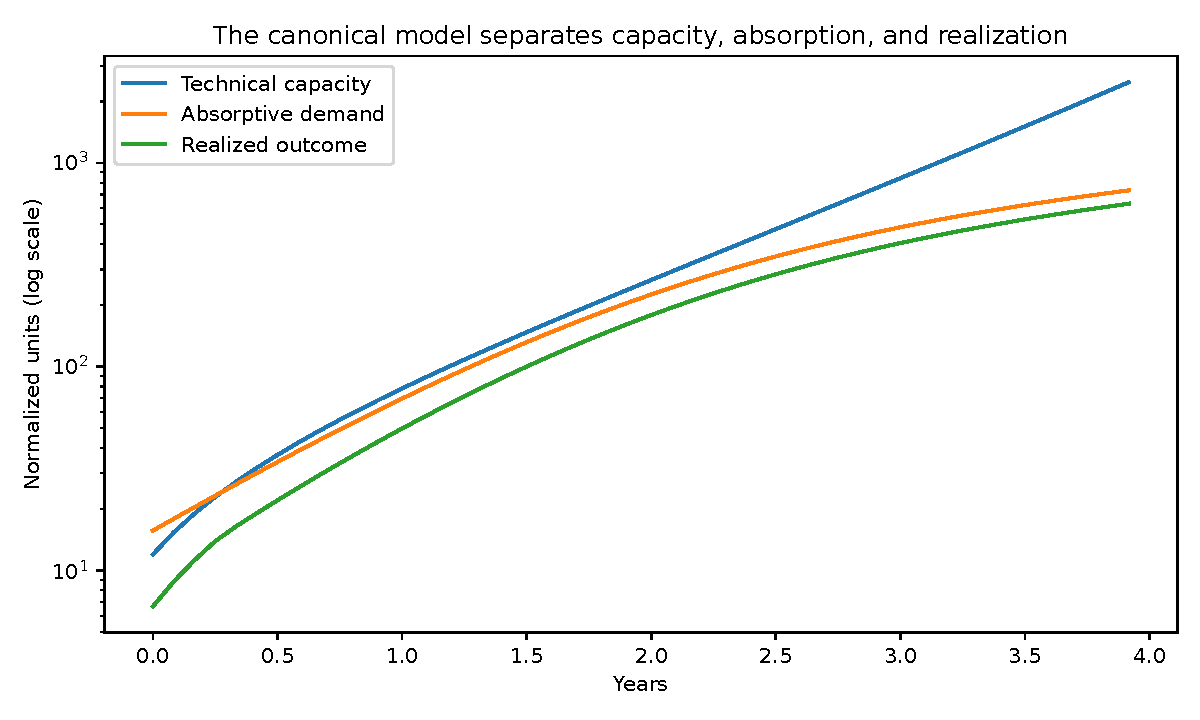
\includegraphics[width=0.88\textwidth]{canonical_branches.pdf}
\caption{Illustrative compact canonical branches. Realized output follows the lower branch and is then reduced by constraints not already represented in that branch. The figure is controlled, not an empirical forecast.}
\label{fig:canonical-branches}
\end{figure}

\subsection{Generalized realization family}

The hard minimum is not the only defensible aggregation law. Some domains permit partial substitution, and constraints can operate asymmetrically on technical supply, absorptive demand, or the transfer between them. Version 2.0.0 therefore embeds Equation~\eqref{eq:canonical} in a generalized constant-elasticity realization family:
\begin{equation}
\label{eq:generalized-realization}
\boxed{
Y_s(t)=B_s^X(t)
\left[
\alpha_s\bigl(B_s^Q(t)Q_s(t)\bigr)^{-\rho_s}
+(1-\alpha_s)\bigl(B_s^Z(t)Z_s(t)\bigr)^{-\rho_s}
\right]^{-1/\rho_s}.}
\end{equation}
Here $B_s^Q$ acts on technical production, $B_s^Z$ acts on absorptive demand, $B_s^X$ acts on realization or transfer, $\alpha_s\in(0,1)$ controls branch weight, and $\rho_s>0$ controls substitutability. As $\rho_s\rightarrow\infty$,
\begin{equation}
Y_s(t)\rightarrow B_s^X(t)\min\{B_s^Q(t)Q_s(t),B_s^Z(t)Z_s(t)\}.
\end{equation}
Equation~\eqref{eq:canonical} is recovered when the branch-specific factors equal one and $B_s^X=B_s$. Finite $\rho$ should be used only when substitution has domain evidence; otherwise the hard minimum is the transparent baseline. The reference engine supports both and requires the operator choice to be recorded.

\subsection{Technical-output decomposition}

The technical-output growth rate is
\begin{equation}
\label{eq:technical-growth}
\boxed{
\begin{aligned}
g_{Q,s}(t)=\;&\beta_\theta\dot\theta_s(t)
-\beta_c\frac{\dot c_s(t)}{c_s(t)}
-\beta_\tau\frac{\dot\tau_s(t)}{\tau_s(t)}\\
&+\beta_A\frac{\dot A_s(t)}{A_s(t)+\varepsilon}
+\beta_P\frac{\dot P_s(t)}{P_s(t)}
+\beta_R\frac{\dot R_s(t)}{R_s(t)}.
\end{aligned}}
\end{equation}
Here $\theta$ is latent capability, $c$ cost per attempt or unit of work, $\tau$ task-completion time, $A$ automatable workflow share, $P$ effective parallelism, $R$ verified reliability, $\beta_j$ target-specific elasticities, and $\varepsilon>0$ a stabilizer.

Equation~\eqref{eq:technical-growth} is an accounting and estimation structure, not permission to set every elasticity to one. Capability, cost, speed, automation, parallelism, and reliability often share causes. Their coefficients are not causally identified by a short aggregate time series. A defensible implementation must estimate them from panel or task-level variation, constrain them using domain knowledge, or declare them scenario assumptions and perform sensitivity analysis.

\subsection{Capability measurement}

Raw benchmark averages saturate and change composition. A latent item-response representation is
\begin{equation}
\Pr(\text{success on item }i\mid t)=\sigma\!\left[a_i(\theta(t)-b_i)\right],
\qquad \sigma(x)=\frac{1}{1+e^{-x}},
\end{equation}
where $b_i$ is item difficulty and $a_i$ discrimination \citep{rasch1980}. For an economically meaningful task, capability becomes deployable only after its success probability, verification burden, failure severity, authority, and cost jointly satisfy the acceptance rule.

\subsection{Residual bottlenecks}

For constraint factors $b_k(t)\in(0,1]$ and weights $w_k\ge0$ summing to one, a smooth weakest-link aggregator is
\begin{equation}
\label{eq:bottleneck}
B_\varrho(t)=\left[\sum_{k=1}^{K}w_k b_k(t)^{-\varrho}\right]^{-1/\varrho},\qquad \varrho>0.
\end{equation}
As $\varrho\rightarrow\infty$, $B_\varrho$ approaches the minimum factor. Smaller $\varrho$ permits several constraints to matter jointly. The notation $\varrho$ is distinct from the realization-family parameter $\rho_s$.

\subsection{Double-counting and dimensional audit}

Every material factor is assigned to exactly one substantive location: technical capacity, absorptive demand, branch-specific bottleneck, or transfer bottleneck. It may additionally appear as a diagnostic but not as a second penalty. If legal authorization is already embedded in eligible adoption $D(t)$, applying the same eligibility fraction again in $B^Z$ is double counting. If workflow reliability already determines cost per verified output, multiplying by that identical reliability again may be inappropriate.

Before fitting, the analyst must also verify dimensional consistency. $Q_s$ and $Z_s$ must be expressed in compatible units and over the same time basis. A stock cannot be minimized directly against a flow without conversion; a probability cannot be multiplied into currency without a defined exposure or quantity; a benchmark percentage cannot be interpreted as mission throughput without a mapping model.

\begin{methodbox}
\textbf{Plain-language interpretation.} Realized output is governed by what can be produced, what can be absorbed, and what can cross the boundary between them. The compact model uses a hard weakest link. The generalized model permits explicit, evidence-backed asymmetry and partial substitution without hiding those choices.
\end{methodbox}


\section{Candidate Growth Regimes and Discontinuities}

No model class is assumed ex ante. The protocol fits or evaluates a family whose members encode different causal stories.

\subsection{Linear and exponential baselines}

\begin{align}
X_L(t)&=X_0+vt,\\
X_E(t)&=X_0e^{gt}.
\end{align}
The linear model is useful as a conservative absolute-change baseline. The exponential model assumes a stable proportional rate.

\subsection{Acceleration and decaying acceleration}

If the proportional growth rate rises linearly, $g(t)=g_0+at$, then
\begin{equation}
\label{eq:accelerating}
X_A(t)=X_0\exp\left(g_0t+\tfrac12at^2\right).
\end{equation}
Constant acceleration is often too aggressive. If acceleration decays as $\dot g(t)=a_0e^{-\kappa t}$, then
\begin{equation}
\label{eq:decay-acc}
X(t)=X_0\exp\left[g_0t+\frac{a_0}{\kappa}t-\frac{a_0}{\kappa^2}\left(1-e^{-\kappa t}\right)\right].
\end{equation}
This model permits current acceleration while making its persistence an estimable parameter.

\subsection{Constrained and moving-ceiling models}

A generalized logistic process is
\begin{equation}
\dot X=rX\left[1-\left(\frac{X}{K}\right)^\nu\right].
\end{equation}
The ceiling $K$ need not be a permanent physical limit. It can represent capacity under the current compute, regulation, capital, demand, or institutional regime. A moving-ceiling model combines acceleration and constraints:
\begin{equation}
\label{eq:moving-ceiling}
\dot X=g(t)X B(t)\left[1-\left(\frac{X}{K(t)}\right)^\nu\right].
\end{equation}

\subsection{Change points and regime switching}

A continuous one-change log-linear model is
\begin{equation}
\ln X(t)=\alpha+g_1t+\Delta g\,(t-\tau)_+ + \epsilon_t,
\end{equation}
where $(x)_+=\max(x,0)$. More general hidden-state models can follow Hamilton-style regime switching \citep{hamilton1989}. Change points are useful for release-driven jumps, benchmark revisions, policy shocks, and new production architectures, but retrospective fit can overstate prospective detectability.

\subsection{Conditional recursive-improvement regime}

Let $A_R(t)\in[0,1]$ be the independently verified and authorized fraction of the AI-improvement loop that operates autonomously. Let $g(t)=\dd\ln X/\dd t$. After transition time $\tau$,
\begin{equation}
\label{eq:recursive-g}
\dot g(t)=\left[\kappa A_R(t)-\delta\right]g(t).
\end{equation}
If $q=\kappa A_R-\delta>0$ is locally constant,
\begin{equation}
g(t)=g_\tau e^{q(t-\tau)}
\end{equation}
and
\begin{equation}
\label{eq:double-exp}
\boxed{X_D(t)=JX(\tau^-)\exp\left[\frac{g_\tau}{q}\left(e^{q(t-\tau)}-1\right)\right].}
\end{equation}
$J\ge1$ is an immediate jump. This double-exponential form is a stress model for a growth rate that compounds; it is not a prediction of infinite physical output. The operational form substitutes $g(t)$ into Equation~\eqref{eq:moving-ceiling} so compute, energy, capital, fabrication, authority, safety, and adoption remain binding where appropriate.

A transition hazard can be tied to observable triggers:
\begin{equation}
\lambda(t)=\lambda_0\exp(\gamma^\top z(t)),\qquad
\Pr(\tau\le T)=1-\exp\left[-\int_0^T\lambda(u)\dd u\right].
\end{equation}
Candidate elements of $z(t)$ include fresh-task autonomous R\&D gains, independently reproduced multi-generation improvements, experiment-loop compression, long-horizon reliability, automated evaluation, deployment authority, and available compute/energy. Precise probabilities are not warranted where these relationships are weakly identified.

\begin{figure}[H]
\centering
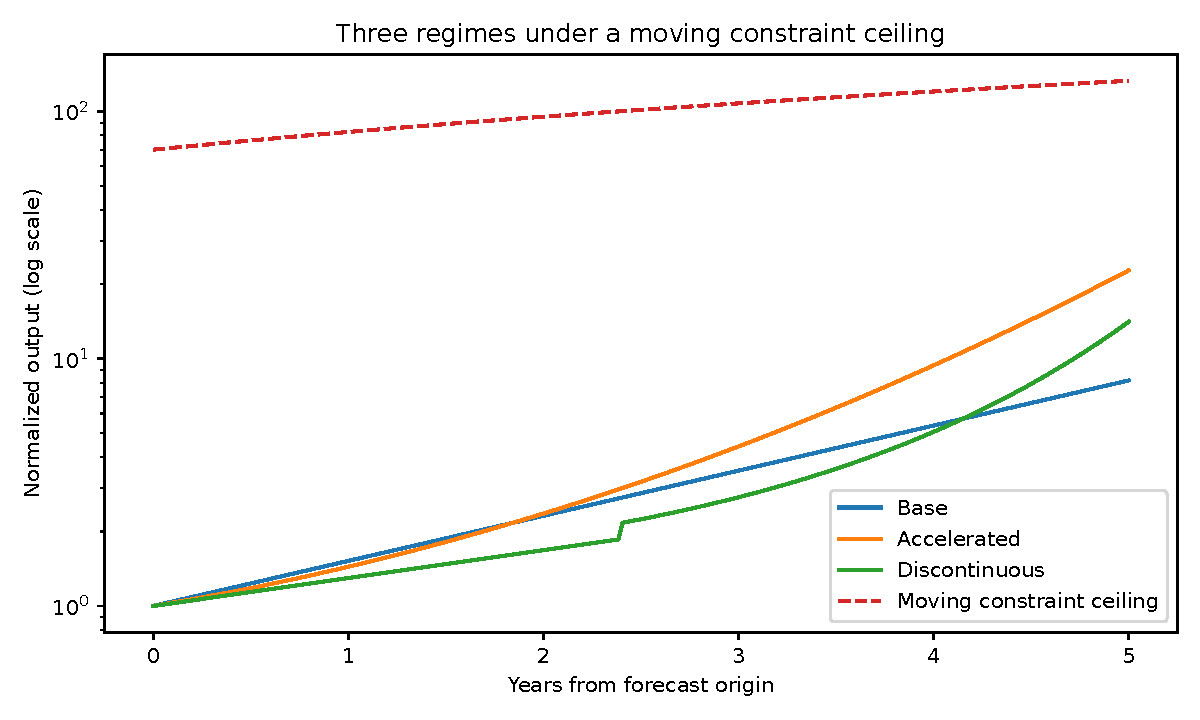
\includegraphics[width=0.88\textwidth]{regime_paths.pdf}
\caption{Controlled examples of linear, exponential, accelerating, constrained, and regime-changing paths. Curves illustrate structural differences; they are not empirical AI timelines.}
\label{fig:regime-paths}
\end{figure}

\subsection{Scenario definitions}

\begin{description}[style=nextline]
\item[Base.] Verified progress continues, some saturation occurs, institutions adjust gradually, and no recursive-improvement transition occurs.
\item[Accelerated.] Recent acceleration is partly persistent; costs, task time, automation, and parallelism improve faster; constraints and adoption respond more quickly, with acceleration allowed to decay.
\item[Discontinuous.] A conditional transition closes a material part of the improvement loop and causes the growth rate itself to compound, while real-world output remains constraint-limited.
\end{description}
Scenarios are reported separately. An expected value alone can hide the asymmetric implications of a low-probability discontinuity.


\section{From Capability to Verified Work}

Historical project duration is not a physical constant. When execution, verification, retries, and parallelism change, the workflow must be recomputed from its current graph $G=(V,E)$.

\subsection{Expected attempts and task duration}

For task $i$, let $p_i$ be autonomous success probability per attempt and $m_i$ the maximum attempts before escalation. The expected number of attempts is
\begin{equation}
N_i^{\mathrm{attempt}}=\frac{1-(1-p_i)^{m_i}}{p_i},
\end{equation}
and escalation probability is $(1-p_i)^{m_i}$. With AI execution time $\tau_i^{AI}$, verification time $\tau_i^V$, human fallback $\tau_i^H$, authority latency $\ell_i^A$, and external latency $\ell_i^E$,
\begin{equation}
\label{eq:task-duration}
\bar\tau_i=N_i^{\mathrm{attempt}}(\tau_i^{AI}+\tau_i^V)+(1-p_i)^{m_i}\tau_i^H+\ell_i^A+\ell_i^E.
\end{equation}
The separation matters: faster inference does not shorten a statutory waiting period, board approval, procurement cycle, laboratory incubation, or physical shipment.

\subsection{Critical path and effective parallelism}

Total expected work and critical path are
\begin{equation}
W=\sum_{i\in V}\bar\tau_i,\qquad
CP=\max_{\pi\in\mathcal P(G)}\sum_{i\in\pi}\bar\tau_i.
\end{equation}
With $n$ workers and parallel-efficiency exponent $\eta\in(0,1]$,
\begin{equation}
\label{eq:workflow-time}
\boxed{T_{\mathrm{workflow}}\approx\max\left\{CP,\frac{W}{n^\eta}\right\}+H_{\mathrm{coord}}(n).}
\end{equation}
This is an Amdahl-style constraint: parallel workers cannot erase a serial critical path \citep{amdahl1967,gustafson1988}.

\subsection{Reliability and verified cost}

If per-attempt verified reliability is $r_i$, then with $m_i$ independent attempts
\begin{equation}
r_i^*=1-(1-r_i)^{m_i}.
\end{equation}
For required steps,
\begin{equation}
\ln R_{\mathrm{workflow}}=\sum_i\ln r_i^*-\Omega_{\mathrm{corr}},
\end{equation}
where $\Omega_{\mathrm{corr}}\ge0$ penalizes common-mode failures. Expected cost is calculated from attempts, verification, and fallback; cost per verified successful workflow is
\begin{equation}
C_{\mathrm{verified}}=\frac{C_{\mathrm{workflow}}}{R_{\mathrm{workflow}}}.
\end{equation}
Raw token price is therefore not the decision-relevant cost when retries, verification, and failure severity dominate.

\subsection{Controlled workflow result}

The reference fixture contains parallel research tasks, a serial synthesis/review/release chain, retries, verification, and coordination overhead. Its total expected work is approximately \SI{14.88}{\hour}, but the critical path is \SI{13.26}{\hour}. Moving from one to two workers reduces duration; adding further workers eventually increases estimated duration because the critical path remains and coordination overhead rises.

\begin{figure}[H]
\centering
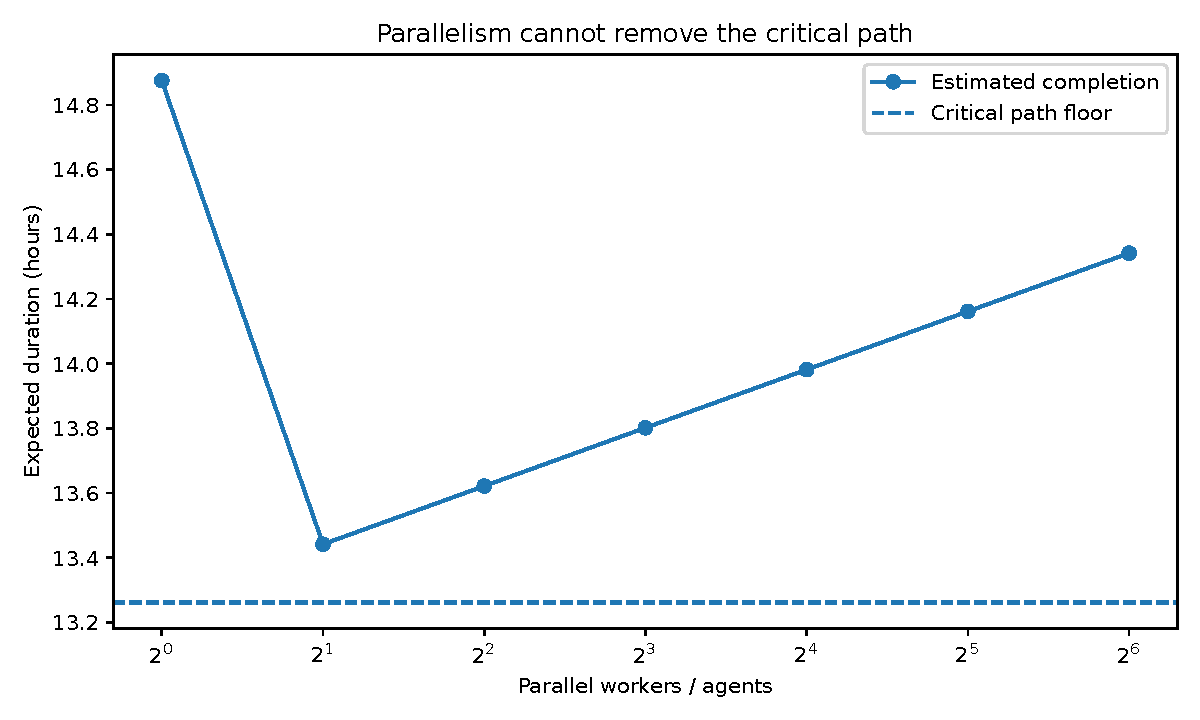
\includegraphics[width=0.84\textwidth]{workflow_parallelism.pdf}
\caption{Controlled workflow duration as parallel workers increase. The critical path prevents unlimited compression; coordination eventually offsets additional parallel capacity.}
\label{fig:workflow-parallelism}
\end{figure}

\begin{table}[H]
\centering
\caption{Selected controlled workflow outcomes.}
\begin{tabular}{rrrr}
\toprule
Workers & Duration (h) & Critical path (h) & Coord. overhead (h) \\
\midrule
1 & 14.88 & 13.26 & 0.00 \\
2 & 13.44 & 13.26 & 0.18 \\
4 & 13.62 & 13.26 & 0.36 \\
8 & 13.80 & 13.26 & 0.54 \\
32 & 14.16 & 13.26 & 0.90 \\
64 & 14.34 & 13.26 & 1.08 \\
\bottomrule
\end{tabular}

\label{tab:workflow}
\end{table}

The separate authority-latency example in the package demonstrates an even stronger case: a 24-hour authorization task dominates a workflow despite rapid machine execution. These examples are mechanical demonstrations, not estimates of a particular organization.

\section{Estimation, Probabilistic Forecasting, and Model Uncertainty}

\subsection{Observation model and comparable likelihoods}

For candidate model $m$ with positive trajectory $f_m(t;\Theta_m)$, a basic log-scale observation equation is
\begin{equation}
\ln y_t=\ln f_m(t;\Theta_m)+\epsilon_t.
\end{equation}
The reference implementation optimizes a Gaussian log-likelihood on log outcomes and counts the residual-scale parameter when calculating information criteria. A robust production analysis may instead use
\begin{equation}
\epsilon_t\sim t_\nu(0,\sigma_m),
\end{equation}
heteroskedastic errors, explicit measurement-error models, or revision processes. Competing models must be compared using likelihoods defined on the same observation scale and data. Mixing least-squares objectives, uncounted change-point searches, and incomparable residual definitions produces misleading information weights.

\subsection{Information criteria and model averaging}

For maximized log likelihood $\hat L_m$, $k_m$ estimated parameters, and $n$ observations,
\begin{equation}
\mathrm{AICc}_m=2k_m-2\ln\hat L_m+\frac{2k_m(k_m+1)}{n-k_m-1}.
\end{equation}
Weights are
\begin{equation}
w_m=\frac{\exp(-\Delta_m/2)}{\sum_j\exp(-\Delta_j/2)},\qquad
\Delta_m=\mathrm{AICc}_m-\min_j\mathrm{AICc}_j.
\end{equation}
The full predictive distribution can average over model and scenario uncertainty:
\begin{equation}
\label{eq:model-scenario-average}
p(Y_T\mid\mathcal D)=\sum_{s\in\mathcal S}\pi_s\sum_mw_{m,s}\,p(Y_T\mid M_{m,s},\mathcal D).
\end{equation}
Model averaging is not automatically superior. Component models can be redundant, misspecified, or unstable outside the identification range. Rolling-origin performance is therefore reported alongside in-sample criteria, and scenario weights are never presented as objective frequencies when they are judgmental decision weights.

\subsection{Residual-bootstrap predictive distributions}

Version 2.0.0 implements a reproducible residual-bootstrap ensemble. For each draw $b$:
\begin{enumerate}
\item select model $m_b$ according to the model weights;
\item resample centered log residuals from $m_b$;
\item refit the selected model to the bootstrap series;
\item predict the requested dates and optionally draw process noise;
\item apply the target bounds, realization operator, and scenario transformation.
\end{enumerate}
The resulting samples $\{Y_s^{(b)}(t)\}_{b=1}^{B}$ generate medians, means, and central 50\%, 80\%, and 95\% intervals. In the technical-to-realized implementation, each draw also propagates disclosed log-scale or logit-scale uncertainty through market size, adoption, utilization, technical constraints, demand constraints, and transfer constraints. This prevents a deterministic active ceiling from collapsing the realized-output interval even when technical-capacity uncertainty is substantial. Common random numbers are used across scenarios so that scenario comparisons are not dominated by unrelated Monte Carlo noise. The implementation currently treats these realization-parameter draws as independent unless a domain-specific model replaces them; that approximation must be disclosed and tested when dependence is material. The procedure captures residual, discrete-model, and declared realization-parameter uncertainty but not every source of structural uncertainty. It is intentionally transparent and replaceable by a Bayesian posterior, block bootstrap, state-space model, copula, or domain-specific simulator.

\subsection{Rolling-origin hindcasting and proper scores}

At historical cutoff $t_k$, only evidence dated at or before $t_k$ may be used to predict later observations. This procedure detects leakage and tests whether a model adapts quickly enough to acceleration, saturation, or a break. Point metrics include log-RMSE, log-MAE, and sMAPE. Probabilistic evaluation uses proper scores \citep{gneiting2007}, including the Brier score
\begin{equation}
\mathrm{BS}=\frac{1}{N}\sum_{i=1}^{N}(p_i-o_i)^2,
\end{equation}
the logarithmic score, the continuous ranked probability score, and interval score. Coverage alone is insufficient: arbitrarily wide intervals can cover everything while providing little information.

\subsection{Uncertainty decomposition}

Total predictive variance decomposes as
\begin{equation}
\Var(Y)=\E_M[\Var(Y\mid M)]+\Var_M[\E(Y\mid M)].
\end{equation}
A complete forecast separately records measurement, parameter, residual, model, scenario, transition-timing, execution, and decision uncertainty. Sensitivity to parameter $\Theta_j$ is
\begin{equation}
S_j=\frac{\partial\ln Y}{\partial\ln\Theta_j}.
\end{equation}
Intervals should widen when evidence is sparse, non-comparable, near a benchmark ceiling, or extrapolated far beyond the observed domain. An external measurement boundary should normally be reported as a boundary, not converted into false certainty by clipping every draw to the same cap.

\subsection{Milestone distributions}

A milestone $M$ is achieved only when output, reliability, and deployability conditions are simultaneously satisfied:
\begin{equation}
T_M=\inf\left\{t:Y(t)\ge M,\;R(t)\ge R_M,\;b_k(t)\ge b_{k,M}\right\}.
\end{equation}
The engine evaluates $T_M$ across predictive samples and returns the probability of crossing by the horizon and conditional crossing-date quantiles. A milestone date with a low crossing probability is not presented as a scheduled fact.

\subsection{Change-point and discontinuity uncertainty}

A selected break date is not known merely because it maximizes an in-sample criterion. Where transition timing matters, the ideal forecast integrates over it:
\begin{equation}
p(Y_T\mid\mathcal D)=\sum_\tau p(Y_T\mid\tau,\mathcal D)p(\tau\mid\mathcal D),
\end{equation}
or uses a hidden-state, survival, or Bayesian change-point model. The reference engine uses a transparent hazard-driven transformation for discontinuity scenarios; it is a stress model, not a claim of calibrated singularity probability.

\section{Reference Engine, Controlled Tests, and Source-Linked Demonstrations}

\subsection{Validation ladder}

The release distinguishes six levels of evidence:
\begin{enumerate}
\item \textbf{L1---mechanical verification:} unit tests, schema validation, deterministic seeds, clean builds, manifests, and checksums;
\item \textbf{L2---controlled mechanism tests:} series generated by known linear, exponential, accelerating, saturating, and change-point processes;
\item \textbf{L3---source-linked historical demonstrations:} frozen excerpts from public primary-source datasets with explicit provenance and limitations;
\item \textbf{L4---preregistered prospective forecasts:} immutable cutoffs, inputs, intervals, triggers, and later scoring;
\item \textbf{L5---independent replication:} a separate team reproduces the software outputs and evaluates the method on unseen targets;
\item \textbf{L6---decision validation:} forecast-guided actions are evaluated against predeclared utility, loss, and regret.
\end{enumerate}
Version 2.0.0 supplies L1--L3 evidence and the registry, templates, and scoring code needed to accumulate L4--L6 evidence. It does not relabel controlled or retrospective demonstrations as prospective validation.

\subsection{End-to-end executable contract}

A single command now transforms a strict schema-valid input into a strict schema-valid probabilistic forecast, a self-contained executive HTML report, milestone crossing distributions, and reproducibility metadata:
\begin{Verbatim}[fontsize=\small,frame=single,breaklines=true]
fwta forecast protocol/v2/examples/canonical-reference-input.yaml \
  --schema protocol/v2/input.schema.json \
  --output results/ceiling/reference-forecast.json \
  --report results/ceiling/reference-forecast.html \
  --output-schema protocol/v2/output.schema.json
\end{Verbatim}
The output records the evidence clock, target semantics, six- and twelve-month pace, model fits and hindcasts, model weights, scenario assumptions and probabilities, interval-valued forecast points, milestones, bottlenecks, triggers, action plan, confidence, recalculation date, engine version, and input hash. A second, explicit 	exttt{fwta register} command can append a frozen output to the hash-chained registry. The release ships an empty live registry and a separately labelled demonstration chain, avoiding any implication that a bundled retrospective example was publicly preregistered.

\subsection{Controlled regime hindcasts}

The deterministic suite generates positive time series under known mechanisms and evaluates multiple candidate models across rolling origins. As expected, linear data favor the linear model and exponential data favor the exponential model. In accelerating and change-point settings, model averaging can perform best over the seeded horizon. In the logistic setting, an accelerating model can temporarily extrapolate well, illustrating a central warning: predictive success over a short window does not identify the true long-run mechanism.

\begin{table}[H]
\centering
\caption{Best rolling-origin model in each controlled generating regime, seed 20260728.}
\begin{tabular}{lll}
\toprule
Generating regime & Lowest-error model & Log RMSE \\
\midrule
accelerating & model average & 0.044 \\
change point & model average & 0.066 \\
exponential & exponential & 0.054 \\
linear & linear & 0.043 \\
logistic & accelerating & 0.058 \\
\bottomrule
\end{tabular}

\label{tab:synthetic-winners}
\end{table}

\begin{figure}[H]
\centering
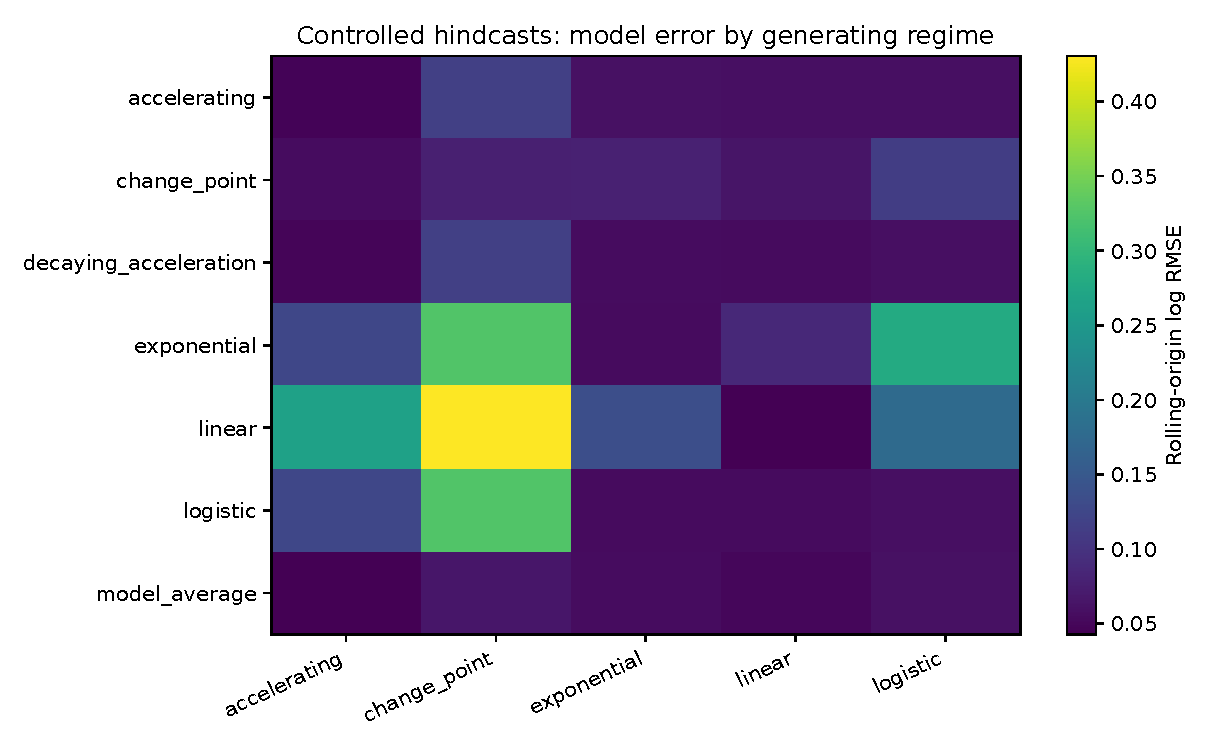
\includegraphics[width=0.88\textwidth]{hindcast_heatmap.pdf}
\caption{Log-RMSE across controlled generating regimes and candidate models. Lower is better. The experiment tests pipeline behavior under known mechanisms, not real-world forecast accuracy.}
\label{fig:hindcast-heatmap}
\end{figure}

\subsection{Canonical-model ablations}

A controlled canonical system is generated with changing capability, cost, time compression, automation, parallelism, reliability, demand, adoption, and bottlenecks. Deliberately removing one or more layers increases forecast error in the seeded system. Because the components are correlated and generated according to the framework, these ablations are integrity tests rather than causal estimates or evidence that the same effect sizes hold in nature.

\begin{table}[H]
\centering
\caption{Controlled canonical-model ablations. Terminal ratio is predicted divided by observed at the final point.}
\begin{tabular}{lrr}
\toprule
Specification & Log RMSE & Terminal ratio \\
\midrule
full canonical & 0.035 & 0.94x \\
no reliability gain & 0.118 & 0.94x \\
no bottlenecks & 0.294 & 1.10x \\
no demand ceiling & 0.481 & 3.20x \\
no automation or parallelism & 0.685 & 0.92x \\
stale constant exponential & 1.334 & 18.98x \\
capability only & 1.459 & 0.19x \\
\bottomrule
\end{tabular}

\label{tab:ablation}
\end{table}

\begin{figure}[H]
\centering
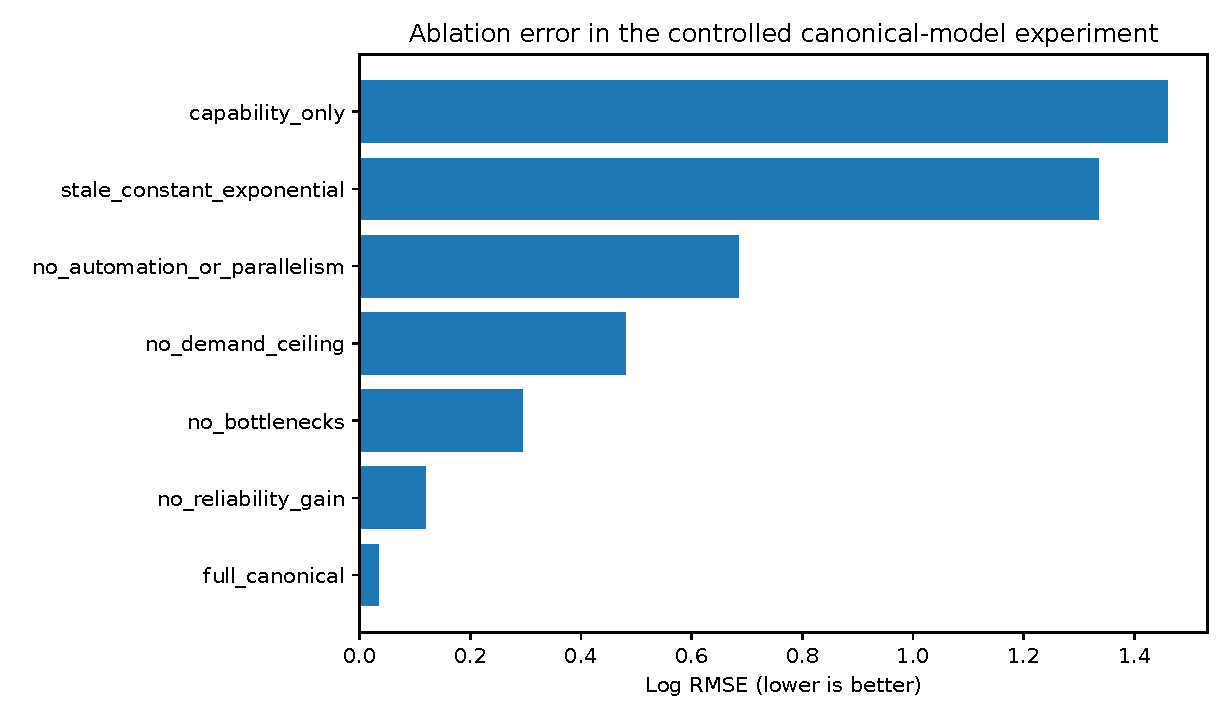
\includegraphics[width=0.88\textwidth]{ablation_error.pdf}
\caption{Controlled ablation error. The exercise demonstrates expected failure modes when structural layers are omitted; it does not estimate real-world elasticities.}
\label{fig:ablation}
\end{figure}

\subsection{Source-linked historical demonstrations}

The first public demonstration uses 13 within-range observations transcribed from METR's Time Horizon 1.1 materials and excludes measurements beyond the stated 16-hour reliability boundary \citep{metr2026}. METR's metric is the human-expert duration of tasks that a system completes at a specified success probability; it is not agent runtime or economy-wide automation. The second demonstration uses seven selected frontier points from the official SWE-bench Verified leaderboard, whose benchmark contains human-validated software issues \citep{jimenez2024,swebench2026}. Both excerpts are frozen with source identifiers and caveats. They are intentionally small and should not be treated as complete mirrors, stable leaderboards, or prospective tests.

\begin{table}[H]
\centering
\caption{Source-linked demonstration summary. The interval shown is the base-scenario 80\% interval at the configured horizon.}
\begin{tabular}{p{0.28\textwidth}rp{0.12\textwidth}rrp{0.20\textwidth}}
\toprule
\textbf{Case} & \textbf{$n$} & \textbf{Best} & \textbf{Log-RMSE} & \textbf{Recent} & \textbf{Horizon median [P80]}\\
\midrule
METR Time Horizon 1.1 excerpt & 13 & change point & 0.292 & 1154.0\% & 960.0 [960.0, 960.0] \\
SWE-bench Verified frontier excerpt & 7 & logistic & 0.019 & 27.7\% & 83.5 [43.6, 86.1] \\
\bottomrule
\end{tabular}
\label{tab:empirical-cases}
\end{table}

\begin{figure}[H]
\centering
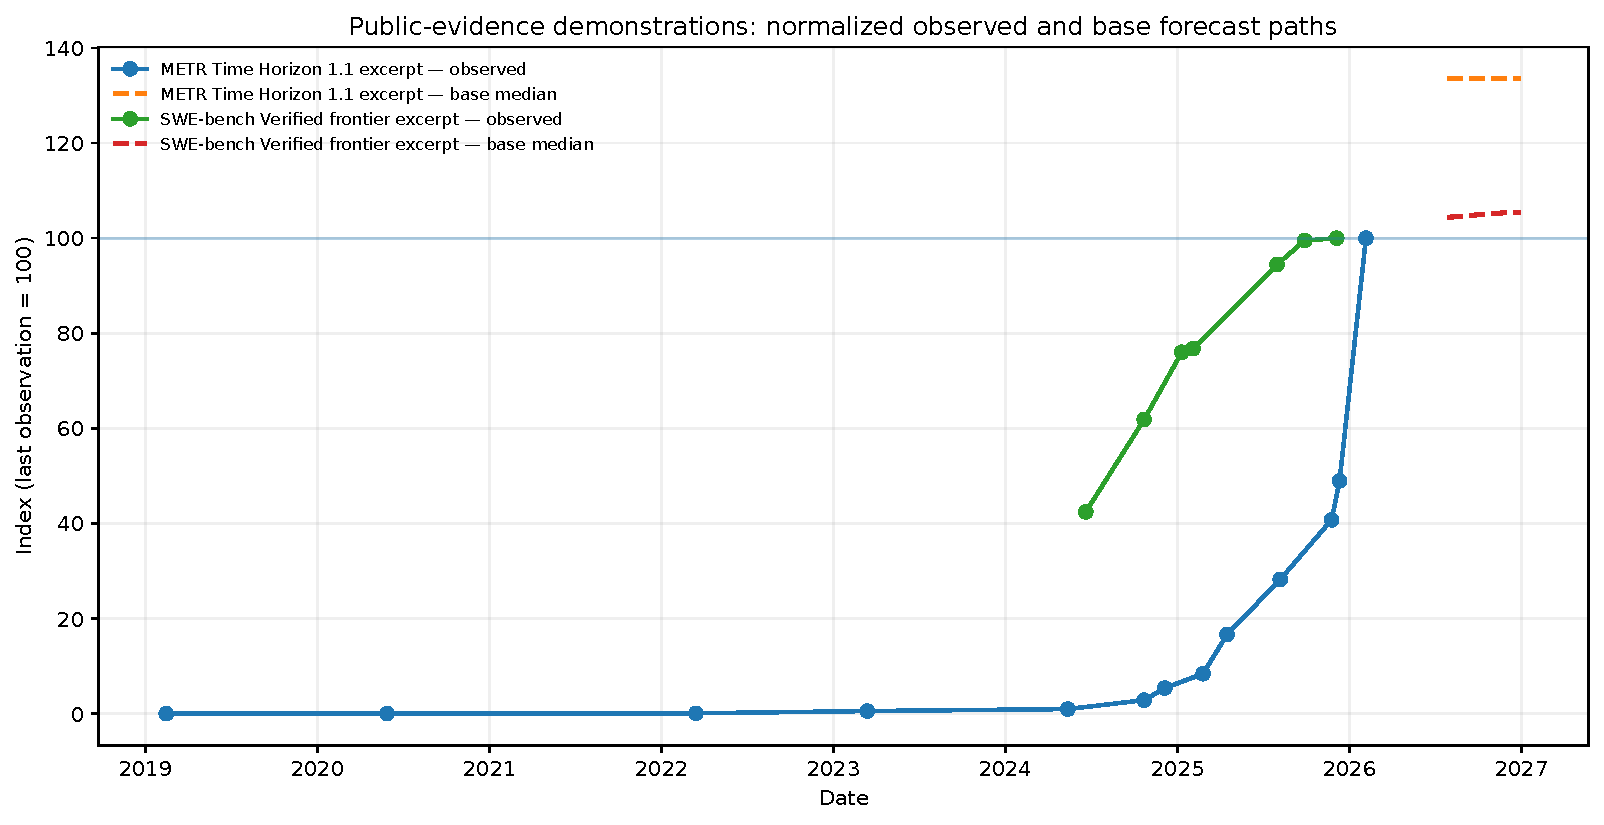
\includegraphics[width=0.94\textwidth]{empirical_cases.pdf}
\caption{Public-evidence demonstrations. METR extrapolation reaches a published measurement boundary; SWE-bench approaches a bounded percentage ceiling. The visualizations exercise different trajectory constraints and do not validate a general AI forecast.}
\label{fig:empirical-cases}
\end{figure}

The METR case illustrates why a measurement boundary must not be mistaken for a physical ceiling. The SWE-bench case illustrates why bounded outcomes require bounded models and why a leaderboard frontier mixes advances in base models, scaffolds, tools, budgets, and attempts. These examples test the data and reporting path; they do not establish causal attribution.

\subsection{Probabilistic rolling-origin scorecard}

Point error alone does not reveal whether uncertainty intervals are useful. We therefore apply six one-step rolling-origin forecasts to the compact within-range METR excerpt and score four predeclared model pools using log-RMSE, the continuous ranked probability score (CRPS), the weighted interval score (WIS), and empirical interval coverage. The sample is too small for general claims, but it exercises the probabilistic path under frozen historical cutoffs. In this run, the full model average has the lowest WIS and CRPS, while the accelerating-only pool has the lowest point RMSE. This disagreement is informative: the model with the best central prediction need not provide the best probabilistic forecast.

\begin{table}[H]
\centering
\caption{Probabilistic one-step rolling-origin hindcasts on the compact METR excerpt ($n=6$ forecast origins). Lower is better for RMSE, CRPS, and WIS. Coverage is descriptive at this sample size.}
\begin{tabular}{lrrrrr}
\toprule
Model pool & RMSE (log) & CRPS & WIS & 80\% cov. & 95\% cov. \\
\midrule
full model average & 0.298 & 45.8 & 138.1 & 83\% & 100\% \\
accelerating only & 0.285 & 49.1 & 145.7 & 100\% & 100\% \\
exponential only & 0.313 & 52.4 & 160.2 & 100\% & 100\% \\
change point only & 0.335 & 61.9 & 176.1 & 67\% & 100\% \\
\bottomrule
\end{tabular}

\label{tab:metr-probabilistic}
\end{table}

\begin{figure}[H]
\centering
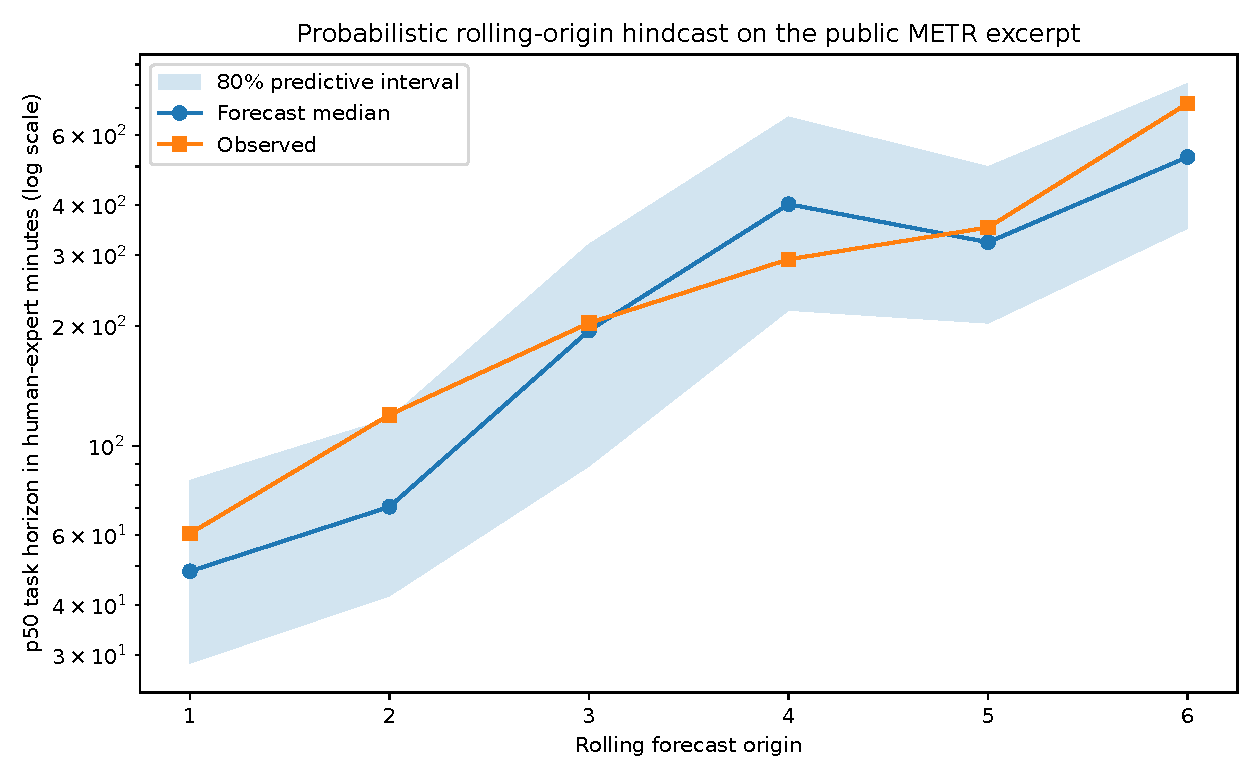
\includegraphics[width=0.88\textwidth]{metr_probabilistic_hindcast.pdf}
\caption{Forecast medians, observed values, and 80\% intervals for the full model-average pool. The logarithmic vertical scale reflects the large dynamic range.}
\label{fig:metr-probabilistic}
\end{figure}

\subsection{Comparability audit: adoption is not one stable series}

The U.S. Census Bureau's Business Trends and Outlook Survey provides an instructive measurement-break case. Earlier releases measured AI use in producing goods or services, while the survey introduced questions about AI use in any business function beginning in November 2025 \citep{census2023ai,census2024btos,census2025history,census2026micro,census2026aiuse}. The broader construct produces a different level and cannot be concatenated mechanically with the earlier series. The release therefore stores the anchors in separate comparability groups and refuses to fit a single adoption trajectory without a validated bridge study.

\begin{table}[H]
\centering
\caption{BTOS AI-use anchors separated by measurement construct. The audit prevents a questionnaire change from being misclassified as adoption acceleration.}
\resizebox{\textwidth}{!}{\begin{tabular}{p{0.27\linewidth}p{0.28\linewidth}rrp{0.22\linewidth}}
\toprule
Comparability group & Construct & First & Last & Decision \\
\midrule
any\_business\_function\_v2 & AI used in any business function & 18.0\% & 19.8\% & Do not splice across the 2025 wording break. \\
goods\_services\_v1 & AI used to produce goods or services & 3.9\% & 10.0\% & Do not splice across the 2025 wording break. \\
\bottomrule
\end{tabular}
}
\label{tab:btos-break}
\end{table}

\subsection{Operational adoption and task compression evidence}

Technical possibility is not realized output, but operational indicators can reveal changing absorption and execution. GitHub reported a rise in average monthly merged pull requests from 35.0 million in 2024 to 43.2 million in 2025, more than one million pull requests created by its coding agent from May through September 2025, and a later change that reduced coding-agent start latency by a reported 50\% \citep{githuboctoverse2025,githubagent2026}. These figures have different denominators and cannot be multiplied into a single productivity index. They are included as evidence that adoption volume and workflow latency have their own clocks and require separate measurement.

\begin{table}[H]
\centering
\caption{Selected operational evidence records retained with source and unit metadata.}
\begin{tabular}{p{0.20\textwidth}p{0.38\textwidth}rp{0.18\textwidth}}
\toprule
\textbf{Period} & \textbf{Metric} & \textbf{Value} & \textbf{Unit}\\
\midrule
2024 & merged\_pull\_requests\_monthly\_average & 35,000,000 & pull requests/month \\
2025 & merged\_pull\_requests\_monthly\_average & 43,200,000 & pull requests/month \\
2025-05 to 2025-09 & coding-agent pull requests created & 1,000,000 & pull requests \\
2026-03-19 & coding-agent start-time improvement & 50\% & fraction faster \\
\bottomrule
\end{tabular}
\label{tab:github-evidence}
\end{table}

\subsection{What the release proves---and does not prove}

The release demonstrates that the equations, schemas, engine, report, registry, controlled experiments, and public-data adapters can execute coherently and reproducibly in the documented environment. It demonstrates that different modelling choices produce materially different forecasts under known mechanisms and on small source-linked series. It does not prove that the canonical model is universally superior, that scenario probabilities are calibrated, that a discontinuity will occur, or that a particular future forecast is correct. Those claims require the prospective and independent program in Section~\ref{sec:validation-program}.


\section{From Forecast to Decision and Recalculation}

\subsection{Action under regime uncertainty}

Let $a$ be an action portfolio and $s$ a scenario with probability or decision weight $\pi_s$. One decision rule is
\begin{equation}
\label{eq:decision}
a^*=\arg\max_a\left\{\sum_s\pi_s\left[\mathrm{NPV}_s(a)+V_{\mathrm{learning},s}(a)+V_{\mathrm{option},s}(a)\right]-\lambda\CVaR_\alpha(L_s(a))\right\},
\end{equation}
subject to budget, authority, reliability, security, legal, and irreversible-loss constraints \citep{rockafellar2000}. When scenario probabilities are too fragile, minimax regret offers a probability-light alternative:
\begin{equation}
a^*=\arg\min_a\max_s\left[V_s^*-V_s(a)\right].
\end{equation}

The preferred present-regime portfolio contains:
\begin{itemize}
\item no-regret actions useful in all scenarios;
\item short, high-information experiments;
\item reversible investments that expand quickly if acceleration triggers fire;
\item pre-authorized capacity, governance, and safety options for discontinuities;
\item delayed irreversible commitments whose value depends on weakly identified tail assumptions.
\end{itemize}

\subsection{Trigger dashboard}

Each trigger has a metric, current value, threshold, source, affected scenario, forecast impact, owner, and required action. Acceleration triggers may include fresh-task gains, falling cost per verified outcome, longer reliable operating horizons, independently reproduced automated R\&D, faster adoption, or compute/energy expansion. Deceleration triggers include reliability plateaus, benchmark contamination, higher verification burden, weak conversion, regulation, incidents, and infrastructure delays.

\subsection{Dated recalculation}

For horizon $H$, the default scheduled interval is
\begin{equation}
\Delta=\min\{30\text{ days},0.1H\}.
\end{equation}
The actual recalculation time is
\begin{equation}
\label{eq:recalc}
t_{\mathrm{recalc}}=\min\left\{t_0+\Delta,T_{\mathrm{forecast\ break}},T_{\mathrm{trigger}},T_{\mathrm{regime\ change}}\right\}.
\end{equation}
A statistical break can be declared when
\begin{equation}
\left|\ln Y_{\mathrm{observed}}(t)-\ln\widehat Y(t)\right|>z_\alpha\sigma_{\mathrm{pred}}(t).
\end{equation}
For a forecast initiated on July 28, 2026, the default monthly date is August 27, 2026 unless $0.1H$ is shorter or a trigger fires first.

\subsection{Revenue specialization}

For sales targets, let $L(t)$ be qualified opportunities, $q(t)$ conversion probability, $\ell(t)$ sales-cycle lag, $V(t)$ average contract value, and $K_{\mathrm{delivery}}(t)$ delivery capacity. Then
\begin{align}
N_{\mathrm{closed}}(t)&=L(t-\ell)q(t-\ell),\\
\mathrm{Bookings}(t)&=V(t)\min\{L(t-\ell)q(t-\ell),K_{\mathrm{delivery}}(t)\}.
\end{align}
For identifiable opportunities, $\E[\mathrm{Bookings}]=\sum_i p_iV_i$. Capability affects revenue only through explicit channels such as lead volume, conversion, cycle time, pricing, delivery, expansion, and retention.

\section{Prospective Validation, Registry, and Independent Replication}
\label{sec:validation-program}

\subsection{Why retrospective fit is insufficient}

A framework designed for regime change can easily overfit a historical narrative. The decisive scientific test is prospective: freeze the evidence, issue the distribution before outcomes are known, preserve the versioned code and assumptions, and score the result after resolution. The repository therefore treats forecasting as an append-only evidence process rather than a sequence of replaceable reports.

\subsection{Hash-chained forecast registry}

Let $F_k$ be the canonical machine-readable forecast record, $h_{k-1}$ the preceding registry hash, and $\mathcal H$ SHA-256. The registry record is
\begin{equation}
h_k=\mathcal H\!\left(\operatorname{canon}(F_k)\,\|\,h_{k-1}\right),
\end{equation}
where $\operatorname{canon}$ is deterministic JSON serialization. Each record includes the forecast identifier, protocol and engine versions, input hash, research cutoff, creation time, previous hash, and current record hash. This detects silent alteration within the published chain. It is not an independent timestamp until the chain is anchored in a public release, archive, or preprint record.

\subsection{Preregistration contract}

Before the forecast origin, a prospective entry should freeze:
\begin{itemize}
\item the target, unit, scope, success definition, and resolution source;
\item the exact evidence cutoff and source snapshots;
\item candidate models, transformations, bounds, and exclusion rules;
\item scenario definitions and whether $\pi_s$ are probabilities or decision weights;
\item interval levels, milestones, triggers, and recalculation policy;
\item primary and secondary scoring rules;
\item allowed corrections and the distinction between an update and a new forecast.
\end{itemize}
The repository supplies a preregistration template and registry verifier. Corrections must append a superseding record; they must not rewrite the prior entry.

\subsection{Independent replication design}

An independent team should receive only the public release and a clean environment. It should verify byte-level artifacts, install the built distribution, reproduce the controlled and public-evidence outputs, rerun the complete forecast command, and document deviations. A stronger replication selects at least one previously unseen target and executes the protocol without assistance from the original author. The replication report should disclose operating system, Python and TeX versions, dependency hashes, command logs, output hashes, and unresolved discrepancies.

\subsection{Decision validation}

Prediction accuracy is not the only objective. For actions $a$ and realized state $s$, define regret
\begin{equation}
\operatorname{Regret}(a,s)=V_s^*-V_s(a).
\end{equation}
Prospective tests should compare the protocol's recommended portfolio with simpler policies such as last-value continuation, constant exponential extrapolation, fixed planning assumptions, and a no-forecast baseline. The framework earns its complexity only if it improves calibration, information value, or decision regret at acceptable operating cost.

\subsection{Publication gates}

The repository uses separate gates for artifact quality and scientific evidence:
\begin{description}
\item[Release gate.] Tests, schemas, end-to-end execution, reproducible paper build, SBOM, checksums, security scan, and legal/IP review checklist pass.
\item[Prospective-evidence gate.] A meaningful set of preregistered forecasts has resolved and been scored.
\item[Validated-method gate.] Results outperform declared baselines across targets, survive independent replication, and remain useful after accounting for operating cost and decision consequences.
\end{description}
Passing the release gate justifies publishing a high-quality research artifact. It does not permit the prospective or validated-method labels prematurely.

\section{Limitations, Falsifiability, and Research Agenda}

\subsection{Identification limits}

Acceleration is difficult to identify from short, revised, selected, and heterogeneous series. A change point can be mistaken for smooth acceleration; a logistic curve can look exponential far below its ceiling; an accelerating curve can mimic bounded growth over a short window. Latent capability, cost, reliability, automation, adoption, and deployment are endogenous and often measured on different task populations. Elasticities in Equation~\eqref{eq:technical-growth} may be weakly identified and correlated. The generalized realization family adds flexibility but also additional identification burden; sensitivity analysis cannot substitute for data.

\subsection{Measurement and comparability}

A recent source can contain an old measurement, and a familiar label can conceal a changed construct. Benchmark suites, scaffolds, elicitation effort, pricing units, business-survey wording, and target populations evolve. The BTOS audit in Section~8 shows that a change from ``producing goods or services'' to ``any business function'' creates a measurement break that should not be interpreted as pure adoption growth. The protocol can flag such breaks, but a valid bridge requires overlapping measurements or a defensible linking model.

\subsection{External validity}

Software tasks with clear tests differ from organizations, scientific laboratories, physical infrastructure, care systems, and regulated decisions. Benchmark task horizon is not wall-clock runtime, and low-context human baselines may not match resident experts. Scaffolds, tools, security constraints, tacit context, and messy environments can materially alter performance. The framework requires domain-specific task graphs and evidence; it is not a universal coefficient table.

\subsection{Distributional uncertainty}

Residual bootstrap intervals inherit the fitted model pool, residual stationarity assumptions, sample size, and historical support. They are not Bayesian posteriors and do not automatically capture unknown unknowns, source revisions, structural breaks outside the candidate set, or strategic behavior. Six METR hindcast origins are far too few for strong calibration claims. Scenario probabilities remain judgmental unless supported by a validated elicitation or event model.

\subsection{Discontinuity uncertainty}

A recursive-improvement regime may not occur, may arrive outside the horizon, may be constrained by evaluation and grounding, or may improve narrow research loops without general transfer. Conversely, sparse monitoring could detect it late. The hazard structure is therefore conditional, not a calibrated probability in the absence of substantial transition data. Double-exponential paths are stress models, not claims of infinite physical output.

\subsection{Prospective and independent validation}

The local package can verify schemas, algorithms, builds, checksums, and frozen demonstrations. It cannot self-certify future predictive accuracy, independent replication, peer review, legal approval, or an external publication timestamp. A live prospective registry becomes scientifically meaningful only when forecasts are committed before outcomes, matured without retroactive editing, and scored by independent parties.

\subsection{Normative and legal limits}

The decision objective embeds values through utility, loss, downside aversion, authority, and constraints. It cannot decide those values neutrally. Forecasts in finance, medicine, law, safety, regulation, employment, or public policy may create professional and statutory duties beyond this research protocol. Repository notices reduce ambiguity but do not eliminate duties, claims, or jurisdiction-specific requirements. Patent, authorship, licensing, privacy, data-use, and publication decisions require qualified review where material.

\subsection{Falsifiable expectations}

The framework should be revised or rejected if, across preregistered targets:
\begin{enumerate}
\item it fails to improve proper scores, calibration, interval coverage, or decision regret over simpler baselines;
\item the canonical branches add complexity without predictive, diagnostic, or decision value;
\item trigger-based updating does not detect breaks faster than fixed schedules;
\item task-graph estimates systematically miss verification, fallback, authority, and external-waiting time;
\item model averaging is persistently worse than robust single-model rules;
\item the generalized family changes decisions mainly through unidentified parameter freedom;
\item independent teams cannot reproduce the controlled and frozen-reference results from the released source;
\item registered forecasts are systematically overconfident or fail to improve after recalibration.
\end{enumerate}

\subsection{Research program}

Priority work includes preregistered rolling hindcasts over multiple targets; reliability-adjusted cost datasets; authority and adoption measurement; bridge studies across changing constructs; causal or bounded estimates of task-level elasticities; hierarchical models across domains; formal double-counting diagnostics; correlated-failure models; transition-hazard elicitation; environment-stable containers; and evaluation of decisions rather than predictions alone. Independent replication, adversarial review, and a public maturity-and-scoring process are essential.

\section{Conclusion}

Forecasts made during accelerating technological change fail when they preserve stale execution assumptions or translate capability directly into realized value. The proposed framework permits acceleration and discontinuity, but forces every projection through evidence comparability, verification, authority, adoption, demand, and residual constraints. It recomputes work from task graphs, compares competing regimes under a common likelihood, propagates uncertainty through full scenario paths, exposes measurement breaks, and converts monitoring into dated action rules.

The compact canonical model is intentionally simple enough to remember:
\[
Y_s(t)=B_s(t)\min\{\text{technical capacity},\text{absorptive demand}\}.
\]
Its disciplined use is not simple. It requires fresh evidence, compatible units, explicit elasticities, a double-counting audit, first-principles execution analysis, calibrated humility about regime transitions, and repeated recalculation. The generalized realization family extends the model only when branch-specific constraints or partial substitution matter enough to justify the added identification burden.

Version 2.0.0 turns the method into a coordinated research system: a complete executable prompt, strict schemas, an end-to-end engine, probabilistic hindcasts, proper scoring, a prospective hash chain, an SBOM, reproducible release machinery, and explicit external validation gates. The package is designed to be falsified and improved, not insulated from evidence.

The central practical instruction remains:

\begin{keybox}
\centering\large\bfseries
Never extrapolate stale timelines. Forecast a world that may accelerate during the forecast itself.
\end{keybox}


\clearpage
\appendix
\section{Complete Executable Reference Prompt}
\label{app:prompt}

This appendix reproduces the complete production reference prompt, version 2.0.0 Ceiling Edition, verbatim. The prompt is an executable natural-language implementation of the paper's protocol; it does not replace the mathematical definitions, code, schemas, evidence, or professional judgment. The canonical standalone files are \texttt{protocol/prompt.md} and \texttt{protocol/prompt.txt}, which are required to be byte-identical at release.

\begin{warningbox}
The prompt requires live evidence when used operationally. Model outputs remain conditional and must not be represented as guaranteed, audited, certified, independently validated, or professionally approved merely because the protocol was followed.
\end{warningbox}

\VerbatimInput[fontsize=\tiny,breaklines=true,breakanywhere=true,frame=single,framesep=2mm,rulecolor=\color{FWLine}]{\ProtocolPath}


\section{Selected Derivations}
\label{app:derivations}

\subsection{Technical capacity from an instantaneous growth rate}

By definition $g_Q(t)=\dd\ln Q(t)/\dd t$. Integrating from 0 to $t$ gives
\[
\ln Q(t)-\ln Q_0=\int_0^t g_Q(u)\dd u,
\]
so
\[
Q(t)=Q_0\exp\left[\int_0^t g_Q(u)\dd u\right].
\]

\subsection{Technical-growth decomposition}

Suppose
\[
Q=Q_0e^{\beta_\theta(\theta-\theta_0)}c^{-\beta_c}\tau^{-\beta_\tau}(A+\varepsilon)^{\beta_A}P^{\beta_P}R^{\beta_R}
\]
up to normalization constants. Taking a time derivative of $\ln Q$ yields Equation~\eqref{eq:technical-growth}.

\subsection{Expected truncated geometric attempts}

For success probability $p$ and maximum $m$ attempts, the number of attempts is at least $k$ with probability $(1-p)^{k-1}$. Therefore
\[
\E[N]=\sum_{k=1}^{m}\Pr(N\ge k)=\sum_{k=1}^{m}(1-p)^{k-1}=\frac{1-(1-p)^m}{p}.
\]

\subsection{Accelerating-exponential crossing time}

Set $M=X_0e^{g_0t+at^2/2}$. Then
\[
\tfrac12at^2+g_0t-\ln(M/X_0)=0.
\]
For $a>0$, the nonnegative root is
\[
T_M=\frac{-g_0+\sqrt{g_0^2+2a\ln(M/X_0)}}{a}.
\]

\subsection{Exponential and logistic crossing times}

For $X=X_0e^{gt}$,
\[
T_M=\frac{\ln(M/X_0)}{g}.
\]
For $X=K/[1+(K/X_0-1)e^{-rt}]$,
\[
T_M=\frac1r\ln\left(\frac{K/X_0-1}{K/M-1}\right),\qquad 0<M<K.
\]

\subsection{Double-exponential crossing time}

From Equation~\eqref{eq:double-exp}, for $M>JX(\tau^-)$,
\[
T_M=\tau+\frac1q\ln\left[1+\frac q{g_\tau}\ln\left(\frac{M}{JX(\tau^-)}\right)\right].
\]

\subsection{Discontinuity hazard}

For a nonnegative time-varying hazard $\lambda(t)$, survival is
\[
S(T)=\exp\left[-\int_0^T\lambda(u)\dd u\right],
\]
so cumulative transition probability is $1-S(T)$.


\subsection{Hard-min limit of the generalized realization family}

Let $x=B^Q Q>0$, $z=B^Z Z>0$, and
\[
G_\rho(x,z)=\left[\alpha x^{-\rho}+(1-\alpha)z^{-\rho}\right]^{-1/\rho}.
\]
Assume without loss of generality that $x\le z$. Then
\[
G_\rho(x,z)=x\left[\alpha+(1-\alpha)(x/z)^\rho\right]^{-1/\rho}.
\]
Since $(x/z)^\rho\to0$ and $\alpha^{-1/\rho}\to1$ as $\rho\to\infty$, $G_\rho(x,z)\to x=\min\{x,z\}$. Multiplying by $B^X$ yields the hard-min limit stated after Equation~\eqref{eq:generalized-realization}.

\subsection{Generalized bottleneck limit}

Equation~\eqref{eq:bottleneck} is a weighted power mean of order $-\varrho$. As $\varrho\to\infty$, the order tends to $-\infty$, whose limit is the minimum component.

\subsection{Workflow reliability}

Independent retry success is one minus the probability all attempts fail: $r_i^*=1-(1-r_i)^{m_i}$. Independent required tasks multiply. Taking logs converts the product to a sum; $\Omega_{\mathrm{corr}}$ subtracts a common-mode penalty.

\subsection{Uncertainty decomposition}

The law of total variance gives
\[
\Var(Y)=\E[\Var(Y\mid M)]+\Var(\E[Y\mid M]),
\]
which separates within-model from between-model uncertainty.


\section{Variable Dictionary}
\label{app:variables}

\small
\begin{longtable}{>{\raggedright\arraybackslash}p{0.14\textwidth}>{\raggedright\arraybackslash}p{0.54\textwidth}>{\raggedright\arraybackslash}p{0.22\textwidth}}
\toprule
\textbf{Symbol} & \textbf{Meaning} & \textbf{Domain / unit}\\
\midrule
\endfirsthead
\toprule
\textbf{Symbol} & \textbf{Meaning} & \textbf{Domain / unit}\\
\midrule
\endhead
$Y_s(t)$ & Realized target outcome under scenario $s$ & Target-specific, nonnegative\\
$Q_0$ & Baseline technically deliverable output & Positive\\
$g_{Q,s}(t)$ & Instantaneous proportional growth rate of technical output & Inverse time\\
$M_s(t)$ & Addressable market, mission volume, or demand pool & Nonnegative\\
$D_s(t)$ & Adoption or penetration fraction & $[0,1]$\\
$U_s(t)$ & Utilization or realized value per adopter & Nonnegative\\
$B_s(t)$ & Compact residual bottleneck factor after double-counting audit & $(0,1]$\\
$B_s^Q(t)$ & Technical-production bottleneck in generalized realization family & $(0,1]$\\
$B_s^Z(t)$ & Absorptive-demand bottleneck in generalized realization family & $(0,1]$\\
$B_s^X(t)$ & Transfer or realization bottleneck in generalized realization family & $(0,1]$\\
$Z_s(t)$ & Absorptive demand, $M_sD_sU_s$ & Same unit as $Q_s$\\
$\alpha_s$ & Branch weight in generalized realization family & $(0,1)$\\
$\rho_s$ & Substitution/weakest-link sharpness in generalized realization family & Positive\\
$\theta(t)$ & Latent capability level & Scale-dependent\\
$c(t)$ & Cost per attempt or unit of work & Positive currency/unit\\
$\tau(t)$ & Task-completion time & Positive time\\
$A(t)$ & Automatable workflow share & $[0,1]$\\
$P(t)$ & Effective parallelism & Positive\\
$R(t)$ & Verified reliability & $(0,1]$\\
$\beta_j$ & Target-specific elasticity of component $j$ & Dimensionless\\
$\varepsilon$ & Stabilizing constant for automation share & Positive, small\\
$b_k(t)$ & Constraint factor $k$ & $(0,1]$\\
$w_k$ & Bottleneck weight & Nonnegative, sums to 1\\
$\varrho$ & Constraint-aggregator sharpness in Equation~\eqref{eq:bottleneck} & Positive\\
$p_i$ & Per-attempt autonomous success probability for task $i$ & $[0,1]$\\
$m_i$ & Maximum autonomous attempts before escalation & Positive integer\\
$\bar\tau_i$ & Expected duration of task $i$ & Time\\
$W$ & Sum of expected task work & Time\\
$CP$ & Expected critical-path duration & Time\\
$n$ & Parallel worker or agent count & Positive integer\\
$\eta$ & Parallel-efficiency exponent & $(0,1]$\\
$H_{\mathrm{coord}}$ & Coordination overhead & Time\\
$\Omega_{\mathrm{corr}}$ & Correlated-failure penalty in log reliability & Nonnegative\\
$A_R(t)$ & Verified and authorized autonomous share of improvement loop & $[0,1]$\\
$\tau$ & Regime-transition time (context-dependent; distinct from task time by subscript) & Time\\
$J$ & Immediate multiplicative jump at transition & $\ge1$\\
$q$ & Post-transition compounding rate of the growth rate & Inverse time\\
$\lambda(t)$ & Transition hazard & Inverse time\\
$K(t)$ & Current regime-dependent ceiling & Positive\\
$\nu$ & Generalized logistic shape & Positive\\
$\pi_s$ & Scenario probability or decision weight & $[0,1]$, sums to 1 when probabilistic\\
\bottomrule
\end{longtable}
\normalsize

\section{Reproducibility and Machine-Readable Protocol}
\label{app:reproducibility}

The canonical repository destination is
\begin{center}
\url{https://github.com/MontrealAI/forecasting-a-world-that-accelerates}.
\end{center}
The URL is a publication target until the repository is actually created and visible. The release never treats a local folder, checksum, or intended URL as an external timestamp.

\subsection{Package map}

\begin{longtable}{p{0.31\textwidth}p{0.59\textwidth}}
\toprule
\textbf{Path} & \textbf{Purpose}\\
\midrule
\texttt{paper/} & LaTeX source, bibliography, generated tables and figures, and compiled preprint.\\
\texttt{protocol/prompt.*} & Complete versioned executable protocol reproduced in Appendix~\ref{app:prompt}.\\
\texttt{protocol/v2/} & Strict version 2 input, output, and registry JSON Schemas plus a complete reference case.\\
\texttt{protocol/variables.yaml} & Canonical variable dictionary and units.\\
\texttt{src/fwta/} & Python implementation of canonical equations, generalized realization, growth models, probabilistic ensembles, scenarios, task graphs, scoring, reporting, registry, and provenance.\\
\texttt{tests/} & Deterministic unit, schema, engine, registry, scoring, workflow, and reproduction tests.\\
\texttt{data/public/} & Frozen source-linked excerpts and controlled fixtures.\\
\texttt{data/provenance/} & Source, retrieval, selection, hash, and limitation records.\\
\texttt{results/ceiling/} & Complete reference forecast JSON and self-contained HTML report.\\
\texttt{results/empirical/} & METR and SWE-bench demonstration outputs.\\
\texttt{registry/} & Hash-chained prospective records, preregistration template, and verification instructions.\\
\texttt{release/} & SBOM, manifest, publication status, release notes, and validation report.\\
\texttt{scripts/} & Build, verification, packaging, repository configuration, and release tools.\\
\texttt{.github/} & CI, compatibility matrix, code scanning, Pages, and draft-release workflows.\\
\bottomrule
\end{longtable}

\subsection{One-command forecast}

After installing the package, a complete reference run is:
\begin{Verbatim}[fontsize=\small,frame=single,breaklines=true]
fwta forecast protocol/v2/examples/canonical-reference-input.yaml \
  --schema protocol/v2/input.schema.json \
  --output results/ceiling/reference-forecast.json \
  --report results/ceiling/reference-forecast.html \
  --output-schema protocol/v2/output.schema.json
\end{Verbatim}
The report is standalone and includes the canonical equations, scenario chart, milestones, bottlenecks, triggers, actions, limitations, and embedded machine-readable output.

\subsection{Clean local reproduction}

\begin{Verbatim}[fontsize=\small,frame=single]
python3 -m venv .venv
source .venv/bin/activate
python -m pip install --upgrade pip
python -m pip install -e '.[dev]'
make verify
\end{Verbatim}
The default tests, controlled experiments, frozen excerpts, and reference forecast require no API key and make no network request. Dependency installation may require network access. The package also supplies a Dockerfile, Compose definition, pinned direct requirements, SBOM generator, Windows instructions, and CI compatibility matrix.

\subsection{Prospective registration}

A completed forecast can be appended to the local registry and verified with:
\begin{Verbatim}[fontsize=\small,frame=single,breaklines=true]
fwta register results/ceiling/reference-forecast.json \
  --registry registry/records.json \
  --record results/ceiling/registry-record.json
fwta registry-verify --registry registry/records.json
\end{Verbatim}
The chain detects mutation within the published sequence. Independent dating requires a public signed release, archival deposit, or preprint service.

\subsection{Release integrity and boundaries}

The release process builds source and wheel distributions, recompiles the paper, validates schemas, reruns experiments, generates a CycloneDX SBOM, scans for common secret patterns, and emits SHA-256 manifests. A checksum proves byte identity with a specified artifact; it does not independently prove authorship, legal priority, non-infringement, or publication time. The publication workflow creates a draft release so an authorized owner can complete the IP and legal gate before public disclosure.


\section{Governance, Use, and Legal Boundaries}
\label{app:governance}

\subsection{License map}

Software is offered under AGPL-3.0-or-later. The paper, prompt, schemas, documentation, and original research artifacts are offered under CC BY-NC-SA 4.0. Third-party material is not relicensed. No trademark license is granted. Separate commercial rights require a signed agreement with MONTREAL.AI. The controlling path-specific map is in \texttt{LICENSE.md}.

\subsection{No warranty or professional opinion}

The framework is research software and methodology. Forecasts are conditional distributions, not promises. They depend on target definition, evidence quality, model choice, parameter estimates, revisions, implementation, and rare events. Users remain responsible for independent verification, professional review where appropriate, authority, data rights, and compliance with applicable law.

\subsection{Contribution controls}

External contributions require DCO sign-off and the project contributor license agreement before merge. The policy preserves provenance, public licensing, coherent commercial licensing, and maintainer control. Contribution does not confer ownership, equity, governance, partnership, agency, employment, or trademark rights.

\subsection{Publication record}

Version 2.0.0 is prepared for the exact standalone repository specified above. At package assembly, the repository and external preprint record had not yet been created. The release documentation prohibits claiming a DOI, cryptographic signature, or public timestamp until the corresponding public record exists.


\clearpage
\bibliographystyle{plainnat}
\bibliography{\PaperRoot/references}
\end{document}
